\section{Rsnap}
\graphicspath{{content/7-solution/3-rsnap/images/}}
\subsection{Implémentation}
Comme expliqué dans la section \ref{Rails}, Rails possède une architecture MVC. Cette section va donc se baser sur sur cette architecture pour présenter la solution proposée.

\subsubsection{modeles}
Les différents concepts utiles pour developper l'application sont ceux représenté par les différents modèles. Ceux-ci sont représenté sur la figure \ref{fig:models}.
\begin{figure}
  \begin{center}
    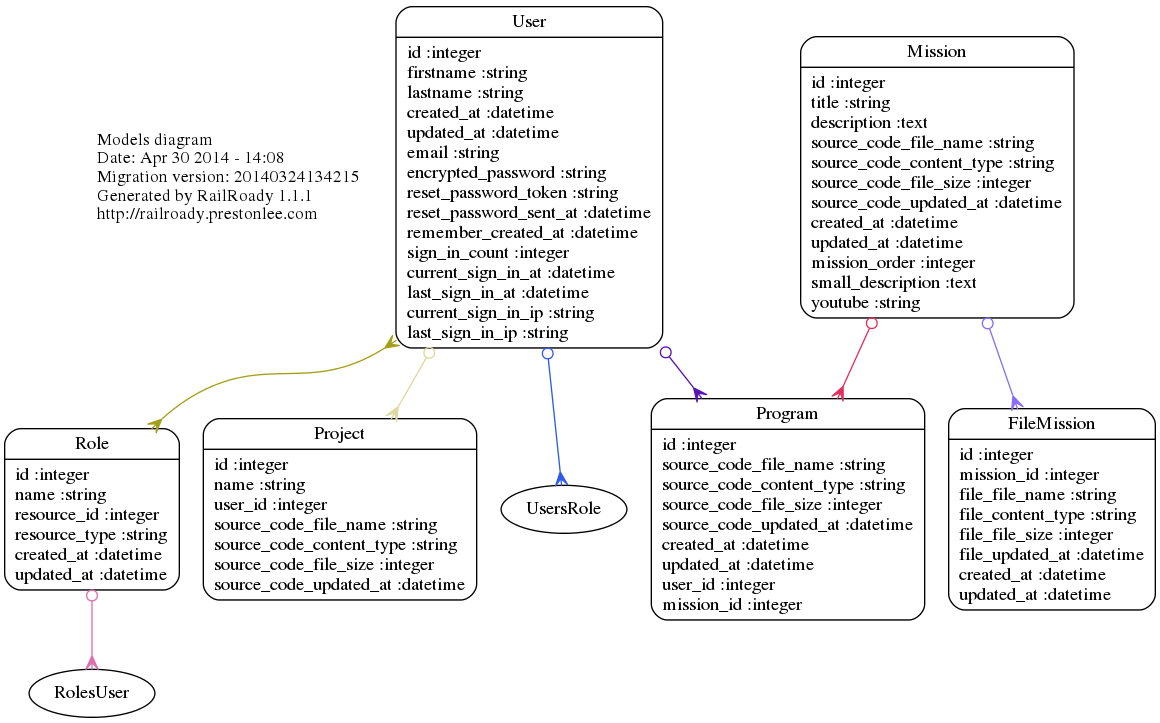
\includegraphics[width=\textwidth]{models_complete}
    \caption{Modèles de Rsnap}
    \label{fig:models}
  \end{center}
\end{figure}
\paragraph{\texttt{User}} L'utilisateur contient les informations nécessaires à l'utiliser (\texttt{firstname}, \texttt{email} \ldots) et les informations pour s'authentifier (\texttt{encrypted\_password}, \texttt{current\_sign\_in\_ip}, \ldots). L'utilisateur peut posséder plusieurs roles, programmes et projets.
\paragraph{\texttt{Role}} Les rôles permettent de donner des attributs à un utilisateur. Ce modèle a été généré automatiquement par Rolify \ref{role}. Dans le cas de Rsnap, Deux rôles ont été créé : \texttt{admin} et \texttt{teacher}. Ces deux rôles sont globaux et donc ne sont pas rattaché à une ressources spécifique.%TODO dans future work: role teacher sur ressource students_group

Les roles seront utiles en conjontion avec les autorités \ref{authority} pour donner des droits supplémentaires à ces type d'utilisateurs.
\paragraph{\texttt{Mission}} Les missions représentent tout ce qui est nécessaire pour avoir un exercice. Un mission comporte donc un titre, une description avec des images et une vidéo pour expliquer à l'étudiant ce qu'il devra faire. Elle comporte en plus le code source initial de l'exercice. Généralement, celui-ci contient les squelette initial du programme pour l'étudiant et les tests pour vérifier le programme. 
\paragraph{\texttt{FileMission}} Les fichiers lié à une mission sont les différentes images que compose la description. %TODO dans furture work : on peut imaginer rajouter la possibiliter de mettre d'autres style de fichier dedans : ex. pdf, slide de cours...
\paragraph{\texttt{Program}} Les programmes comportent les solutions des étudiants à une mission donnée. Il comporte uniquement le code source de l'étudiant.
\paragraph{\texttt{Project}} Les projets sont identique à un programme excepté qu'ils ne sont pas lié à une mission. Il comporte donc le nom du projet en plus du code source.

\paragraph{Exemple} \texttt{Program} est un bon exemple de modèle Rails (code source \ref{lst:model-program}). Seul les fonctionnalités que Active Record \ref{active-record} ne sait pas déduire de lui-même sont présentes. Le modèle contient donc uniquement :
\begin{itemize}
  \item le nom des modèles avec qui il est associé et la cardinalité de la relation (\texttt{belong\_to}) ;
  \item la validation de certains attributs pour qu'ils respectent certaines contraintes (\texttt{validate}) ;
  \item des méthodes de classes pour simplifier les requêtes au modèle (\texttt{scope}, \texttt{self.*}).
\end{itemize}

Comme c'est visible dans les \texttt{scope}, Active Record permet de faire des requêtes SQL directement en Ruby. 
\lstinputlisting[language=Ruby, firstline=21, caption={Modèle \texttt{Program}}, label=lst:model-program]{content/7-solution/3-rsnap/program.rb}

\subsubsection{Controlleurs}
Les contrôleurs donnent accès à différentes ressources. La figure \ref{fig:controllers} montre la liste des contrôleurs implémenté pour l'application. La majorité de ceux-ci se rapporte directement à un modèle spécifique. Il existe néanmoins certaines ressources différentes tel que : 
\begin{itemize}
  \item les pages statiques (\texttt{HomeController}) ;
  \item l'ordonnancement des missions (\texttt{SortMissionsController}) ; 
  \item la création d'un programme depuis une mission (\texttt{InitializationMissionController}) ;
  \item les ressources utile à l'affichage de Snap! (\texttt{SnapAssetsController}).
\end{itemize}
\begin{figure}
  \begin{center}
    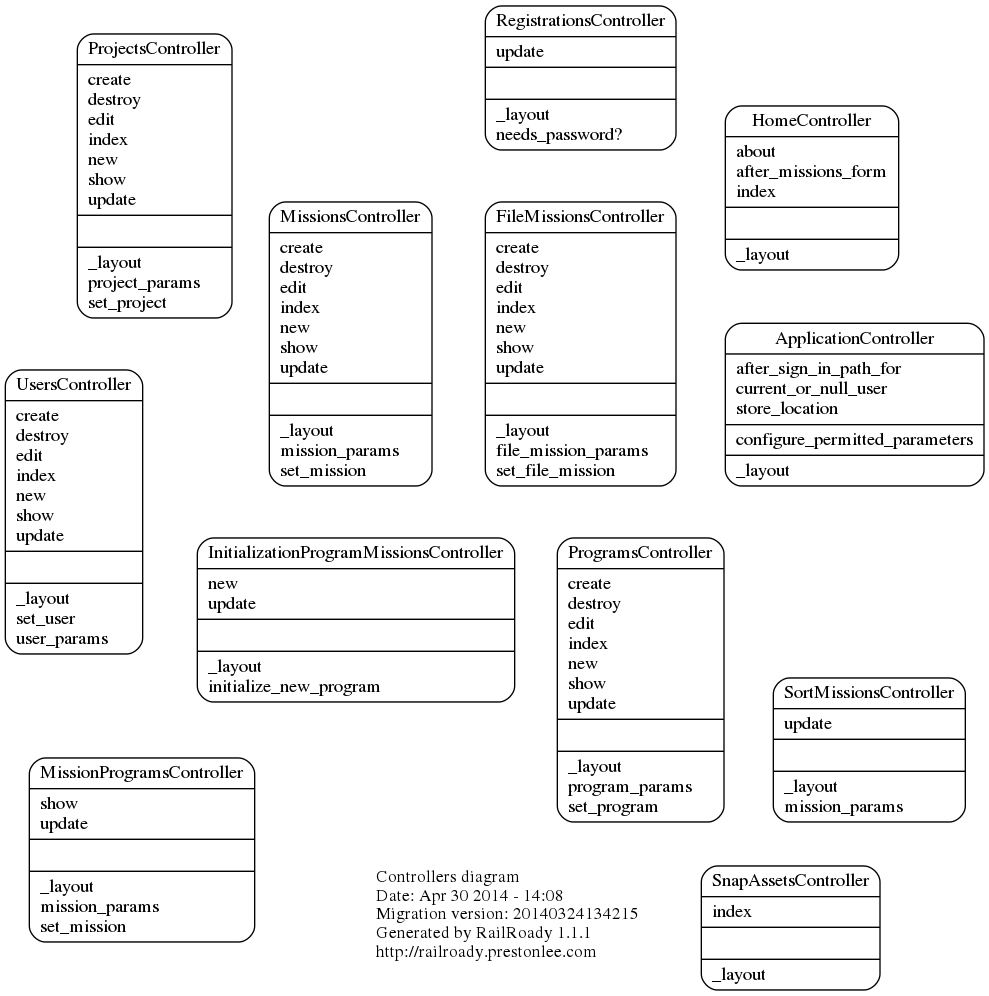
\includegraphics[width=\textwidth]{controllers_complete}
    \caption{Controlleurs de Rsnap}
    \label{fig:controllers}
  \end{center}
\end{figure}

Comme expliqué dans la section \ref{controller}, les méthodes accessibles sont définie dans \texttt{routes.rb}. Les controlleurs ont des tous des ressources RESTfull excepté \texttt{HomeController}. Ceci est visible dans \texttt{routes.rb} ou en regardant les fonctions publiques disponible dans les controlleurs sur la figure \ref{fig:controllers}.

\begin{otherlanguage}{english}
\lstinputlisting[language=Ruby, caption={Controlleur \texttt{MissionsController}}, label=lst:controller-mission]{content/7-solution/3-rsnap/missions_controller.rb}
\end{otherlanguage}

\begin{itemize}
  \item expliquer en pratique comment il sont utilisé
  \item expliquer ce que sont de authority +exemple
  \item montrer pouquoi on retourne parfois du json
  \item montrer ce qu'est un controlleur a la ressource différente du modèle
  \item RESTfull
\end{itemize}

\subsubsection{Vue}
\begin{itemize}
  \item montrer la force de haml avec bootstrap
  \item montrer "render aCollection"
  \item montrer "render aPartial"
  \item montrer utilisation de javascript
\end{itemize}

exemple récapitulatif pour toutes les fonctionnaliés atypique: sort mission

\subsection{Choix tecniques}
expliquer les différentes possibilité de stockage(fichier et site) prix, fonctionnalité...

\subsection{Interface}
présentation de l'interface :
\begin{itemize}
  \item design joli et adaptative
  \item student side
  \item prof side
  \item arrangement des missions + ouverture successive
  \item passage rsnap/snap
\end{itemize}
